\documentclass{beamer}

\mode<presentation>
{
    \usetheme{Madrid}      % or try Darmstadt, Madrid, Warsaw, ...
    \usecolortheme{beaver} % or try albatross, beaver, crane, ...
    \usefonttheme{default}  % or try serif, structurebold, ...
    \setbeamertemplate{navigation symbols}{}
    \setbeamertemplate{caption}[numbered]
}

\usepackage[english]{babel}
\usepackage[utf8x]{inputenc}
\usepackage{amsmath}
\usepackage{graphicx}

\title[NNMF]{Neural Network Matrix Factorization}
\subtitle{\tiny (paper written by: GK Dziugaite, DM Roy, 2015)}
\author[Dmitrii Meinster]{Dmitrii Meinster}
\institute[HSE, CS faculty, DS]{NRU HSE, CS faculty, Data Science programme}
\date{20.12.2017}

\begin{document}

\begin{frame}
  \titlepage
\end{frame}

\begin{frame}{Matrix factorization problem (MF)}
    \begin{itemize}
        \item Suppose we have some big matrix, $X \in \mathbb{R}^{N \times M}$, but only $X_{ij \in J \subset [1..N] \times [1..M]}$ are known.
        \item Want to find $U \in \mathbb{R}^{D \times N}, V \in \mathbb{R}^{D \times M}$, such that: $D \ll N, M; X \approx U^T V$.
        \item Possible applications: collaborative filtering, knowledge graphs
    \end{itemize}
\end{frame}

\begin{frame}{Probability matrix factorization (PMF)}
    (R. Salakhutdinov, A. Mnih, 2008)

    \begin{itemize}
        \item Assume $X_{ij} \sim \mathcal{N}([U^TV]_{ij}, \sigma^2)$
        \item Find $U$ and $V$ by minimizing $\|U^TV - X\|_{F}$
        \item Very effective in practice, but can be further improved
        \item BiasedPMF (Koren et. al., 2009): $X_{ij} \sim \mathcal{N}([U^TV]_{ij} + \mu_i + \tau_j + \beta, \sigma^2)$
    \end{itemize}
\end{frame}

\begin{frame}{PMF note}
    \begin{itemize}
        \item Assume $f(w_1, w_2, \ldots) = \sum_j w_j$
        \item PMF finds mean of $X_{ij}$ \newline in form of $f(U_i \circ V_j)$ (elementwise product of D-dimensional vectors)
        \item Similary, in BiasedPMF, mean of $X_{ij}$ is modeled by $f(U_i \circ V_j, \mu_i, \tau_j, \beta)$.
        \item What if we learn $f$ instead of explicitly defining  it?..
    \end{itemize}
\end{frame}

\begin{frame}{NNMF model}
    \begin{itemize}
        \item Again, $X \in \mathbb{R}^{N \times M}$ with some unknown elements ($J$ --- set of known ones)
        \item To each row $n \in [1..N]$, associate latent feature vector $U_n \in \mathbb{R}^D$ and latent feature matrix $U'_n \in \mathbb{R}^{D' \times K}$
        \item Similarly, for each column  $m \in [1..M]$, we have feature vector $V_m \in \mathbb{R}^D$ and latent feature matrix $V'_m \in \mathbb{R}^{D' \times K}$
        \item $U'_{n, i}$ --- i'th row of matrix $U'_n$ ($K$-dimensional vector); similar for $V'_m$.
        \item (U, V) --- collection of all latent features
        \item Find $\hat{X}_{nm}$ in form of $f_{\theta}(U_n, V_m, U^{'}_{n,1} \cdot V^{'T}_{m,1}, U^{'}_{n,2} \cdot V^{'T}_{m,2}, \ldots)$, where \newline $f_{\theta}$ is function computed by neural network with set of weights $\theta$.
    \end{itemize}
\end{frame}

\begin{frame}{Learning}
    \begin{itemize}
        \item Minimize objective:
        \begin{align*}
            \sum\limits_{(n, m) \in J} (X_{nm} - \hat{X}_{nm})^2 &+ \lambda \Bigg[ \sum\limits_{n} \|U'_n\|^2_F + \sum\limits_{m} \|V'_m\|^2_F \\
            & + \sum\limits_{n} \|U_n\|^2_2 + \sum\limits_{m} \|V_m\|^2_2 \Bigg]
        \end{align*}
        \item On each step, alternate between optimizing neural network weights and the latent features;
        \item RMSProp was used.
    \end{itemize}
\end{frame}

\begin{frame}{Related work}
    \begin{itemize}
        \item Random Function Model (RFM) (Lloyd et al., 2012): gaussian process instead of NN;
        \item Neural Tensor Network (NTN) (Socher et al., 2013): single-layer NN with third-order tensor instead of matrix; first layer of NNMF can be expressed in this form;
        \item Local Low Rank Matrix Approximation (LLORMA) (Lee et al., 2013): approximate each entry by (unique) combination of low-rank matrices;
        \item Restricted Boltzmann Machine (I-RBM) (Salakhutdinov et al., 2007);
        \item I-AutoRec (Sedhain et al., 2015): use autoencoder to generate full matrix from observed ratings; current state-of-the-art for such tasks.
    \end{itemize}
\end{frame}

\begin{frame}{Results}
    $K = 1, D' = 60, D = 10$, each hidden layer contained 50 (for 3HL) or 20 (for 4HL) units.

    \center 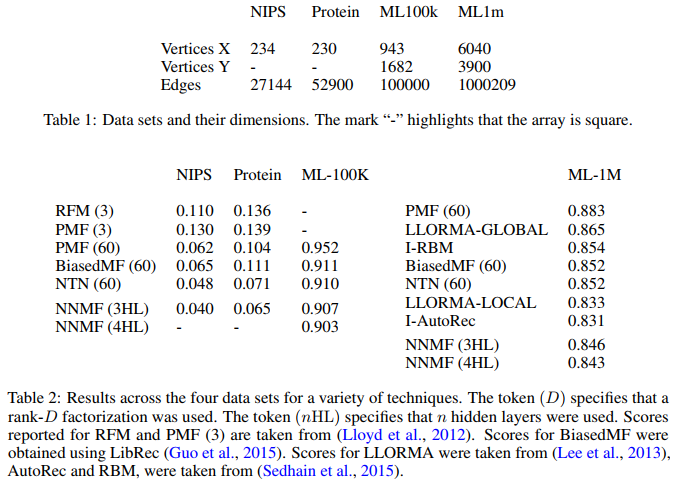
\includegraphics[width=0.8 \textwidth]{results}
\end{frame}

\begin{frame}{Discussion}
    \begin{itemize}
        \item NNMF beats latent feature models, but dominated by approaches which use local graph structure
        \item Further improvements are possible by optimizing NN structure
    \end{itemize}
\end{frame}

\begin{frame}{Thanks!}
    \center Questions?
\end{frame}

\end{document}
